\documentclass{article}

\usepackage[margin=1in]{geometry}
\usepackage{amsmath}
\usepackage{graphicx}  % needed for figures

\title{Formalizing the ATM problem}
\author{Bryan O'Gorman, Tobias Stollenwerk}
\date{\today}

\begin{document}
\maketitle

These notes attempt to formalize the ATM problem: given a set of flights, schedule them in a way that minimizes cost.

\section{Configuration space}

At the highest level, the configuration space is a set of 4D trajectories, one for each flight.
Even with relatively coarsely discretized spacetime, that space is infeasably large.
Therefore we parameterize each trajectory by its deviations from the ideal, conflict-ignorant one.
Such deviations are of two types: temporal and spatial. 
A temporal deviation is simply a delayed start (typically on the order of up to 30 minutes). 
We assume that within the time-scale of such delays, the ideal conflict-ignorant trajectory is time-independent.
There are two types of spatial deviations: global and local.
A global spatial deviation changes the entire trajectory.
For example, one parameterization of global spatial deviations treats each trajectory as an arc in a plane perpendicular to the ground and considers smooth one-parameter curves to the projection of the trajectory onto the ground.
A local deviation consists of a set of maneuvers that change relatively small parts of the spatial trajectory.
Such maneuvers may introduce a delay, but, as with the delays due to temporal deviations, we assume that the subsequent trajectory is unaffected other than simply being delayed.

Henceforth, we focus on origination delays (temporal deviations) and maneuvers (local spatial deviations), because they seem most conducive to quantum annealing.

\section{Cost function}

In reality, the cost function results from factors such as fuel, labor, time, etc.; here we treat it as a unitless quantity that appropriately weights these factors.
Because we are interested in the relative costs of different configurations, we treat the cost of the configuration in which all flights are routed along their independently optimal trajectories, ignoring conflicts, and are exactly on time, as zero.
We further assume that the total cost is the sum of two different types of costs:
\begin{itemize}
  \item for each flight $i$, the cost $c_i^{\mathrm{late}}$ of being late on arrival,
  \item for each pair of flights $\{i, j\}$, the cost of avoiding all conflicts between them 
$c^{\mathrm{avoid}}_{ij} = \sum_{k} c^{\mathrm{avoid}}_{ijk}$, 
which we treat as the sum of the costs of actively avoiding all potential collisions (indexed by $k$).
\end{itemize}
The total cost therefore is 
\begin{equation*}
c = 
\sum_i c^{\mathrm{late}}_i + 
\sum_{ij} \sum_{k \in K_{ij}} c^{\mathrm{avoid}}_{ijk}
,
\end{equation*}
where each contribution to the cost function depends (implicitly as written so far) on the configuration space.
Henceforth, we simplify things by ignoring the direct cost of the local maneuvers. 
However, they will still indirectly contribute to the cost function via their introduction of further delays.
The quantity to minimized can then be written
\begin{equation*}
c = 
\sum_i c^{\mathrm{late}}_i (D_i),
\end{equation*}
where $D_i = d_i + \sum_k d_{ik}$ is the delay of flight $i$ at its destination, which will be a function of its origination delay $d_i$ and delays $d_{ik}$ introduced by local maneuvers.

Lastly, we simplify things further by assuming that all destination delays are equally important (which comes by necessity from the absence of information to the contrary), so that the quantity to minimize is simply the total delay of all flights:
\begin{equation*}
c = D = \sum_i D_i.
\end{equation*}

\section{Classical subroutines}
We further assume the availability of the following two subroutines, whose resource requirements we regard as negligible:
\begin{itemize}
\item given a flight (its origin and destination, and properties of the plane), return the optimal route
\item given two flight paths, return the set of conflicts
\item given two flight paths and start times, and one of the conflicts from above, return the minimum cost of avoiding the conflict (and maybe the induced delay if we allow that)
\end{itemize}

\section{Assumptions made}
\begin{itemize}
\item For each flight, the optimal route is time-independent (both spatially and in duration) over the timescale of possible delays.
For example, if the flight has no potential collisions, its lateness on arrival will exactly equal its departure delay.
\item Actively avoiding a collision (rather than avoiding via departure delays) does not change the cost of actively avoiding other collisions on the same flight path. In reality, one could reason, e.g. that the little bit of fuel used in each active collision avoidance could add up to a disastrously empty tank, but in general we would like the effect of active collision avoidances to be as little as possible.
Similarly, one could argue that the plane burns fuel while idling.
\end{itemize}

\section{Potentially helpful assumptions}
\begin{itemize}
\item All conflicts are pairwise. That is, when two planes have a potential conflict, there are no other planes nearby. 
Furthermore, when this conflict is avoided, it does not create a conflict with another flight. 
(This may be the most unreasonable assumption, e.g. near major airports.)
\item Collisions are symmetric. That is the cost of avoiding them is a function only of the magnitude of the difference in delays of the two flights up until that point. For example, the cost of avoiding a collision between $i$ and $j$ is the same whether $i$ is delayed by $d$ or $j$ is.
\item The lateness cost functions are non-decreasing; we might as well allow it to be negative for earliness, though that could be compiled away by pushing the range of available departure times earlier.
\end{itemize}

\section{Towards a solution}\footnote{
It remains to be proven that this problem is hard, either in general or for realistic values of its parameters (e.g. cost functions).}

\subsection{Sparse case}

First, we describe a method for solving the ``sparse'' version of the problem. 
By sparsity, we mean that all conflicts are between only two trajectories and that no other trajectories are nearby in spacetime, so that potential maneuvers for avoiding a conflict between two flights do not introduce additional conflicts with other flights.

Let $D_{ik} = d_i + \sum_{k' < k} d_{ik}$ be the delay of flight $i$ when it reaches potential conflict $k$.

The delays $(d_{ik}, d_{jk})$ introduced by maneuvering to avoid conflict $k$ between flights $i$ and $j$ is solely a function of the delays $(D_{ik}, D_{jk})$ of those flights up until the conflict and the maneuver $a_{ijk}$ chosen to avoid the conflict.
In particular, the delay depends only on the difference of the delays $\Delta_{ijk} = D_{ik} - D_{jk}$.
It's plausible to assume that it furthermore depends only on the magnitude of this difference $|D_{ik} - D_{jk}|$, though it's not yet clear that that will help.

In general, the avoidance delays as a function of this difference $\Delta_{ijk}$ will be a function of the specific maneuvers chosen. 
We assume, for a given $\Delta_{ijk}$ that there is a minimal delay of each flight $d_{ik}^*$ assuming that the other is unchanged, and that there is a concave ``delay frontier'' in the region $[0, d_{ik}^*] \times [0, d_{jk}^*]$ connecting $(d_{ik}^*, 0)$ and $(0, d_{jk}^*)$ that gives the possible delays $(d_{ik}, d_{jk})$. 
We parameterize this curve by $a_{ijk} \in [0, 1]$.
More generally, there is a ``delay surface'' when various values of $\Delta_{ijk}$ are considered.

We can make several simplifying assumptions of doubtful validity.
One is that we can pick some optimal $a_{ijk}$, so that the delays at collision $k$ depend only on $\Delta_{ijk}$.
Another is to suitably parameterize the ``delay surface'' so that the cost function is simple enough to write a QUBO for.\footnote{TODO}

In the case where maneuvers do not introduce any further delays, we have
\begin{equation*}
c = 
\sum_i c^{\mathrm{late}}_i (d_i) + 
\sum_{ij} \sum_{k \in K_{ij}} c^{\mathrm{avoid}}_{ijk} (d_i, d_j)
=
\sum_i c^{\mathrm{late}}_i (d_i) + 
\sum_{ij} \sum_{k \in K_{ij}} c^{\mathrm{avoid}}_{ijk} (|d_i - d_j|),
\end{equation*}
where $K_{ij}$ is the set of possible collisions between $i$ and $j$.
This form invites a nice QUBO: discretize the each $d_i$, have a bit for each discrete value, enforce that exactly one of them is set, and replace each function above with a sum over the discretized domain of the appropriate quadratic monomials.

\subsection{Dense case}
The sparsity condition assumed above is in general false, even when ignoring near-airport trajectories.

The other extreme is the ``dense'' case, in which all flights are restricted to a ``highway'' as in Olga's thesis.
An appropriate QUBO for that problem is relatively straightforward, and can be written explicitly if needed.

\subsection{General case}
General instances fall into neither of the above extremes.
One potential solution is to use some sort of master-slave subproblem decomposition to combine solvers for each extremal case into a general solution.

\section{Separating spatial and temporal conflicts}
The flights are indexed by
\begin{equation*}
    i \in \{i, \dots, n\}
\end{equation*}
For each flight $i$, the wind-optimal trajectories are given as a sequence of 4-dimensional space-time points
\begin{equation*}
    \tau_i = \{p^i_1, \dots, p^i_{M_i}\}
\end{equation*}
with
\begin{equation*}
    p^i_j = (\mathbf{r}^i_j, t^i_j \Delta_t) = \left( \underbrace{x^i_j \Delta_\text{lat}, y^i_j \Delta_\text{lon}, z^i_j \Delta_v}_{=:\mathbf{r}^i_j}, t^i_j \Delta_t\right)
\end{equation*}
The sequence of points in space are given by
\begin{equation*}
    r_i = \{\mathbf{r}^i_1, \dots, \mathbf{r}^i_{M_i}\}
\end{equation*}
Conflicts may occur if multiple flight trajectories
\begin{equation*}
    \{\tau_i : i \in I_k \subseteq \{1, \dots, n\}\}
\end{equation*}
become to close to each other in time and space.
In the following, we will reduce the multiple flights involved in a given conflict to pairwise conflicts.
With this, a conflict always involves only two flights.

\subsection{Spatial conflicts}
Given the trajectories we can calculate all the spatial conflicts.
The existence of a real conflict depends on the arrival time of both flights $i$ and $j$ at the conflict $k$, $T_{ik}$ and $T_{jk}$ (see figure \ref{fig:spatial_conflicts}). 
The corresponding departure times from the conflict are denoted by 
\begin{equation*}
    T'_{ik} = \frac{L_k}{v_i} + T_{ik}
\end{equation*}
where $L_k$ spatial length of the conflict $k$ and $v_i$ is the constant velocity of flight $i$.
\begin{figure}[htpb]
    \centering
    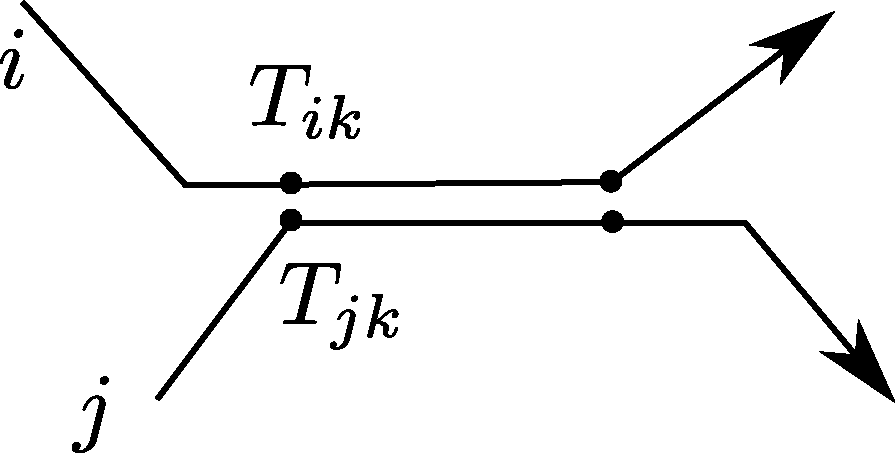
\includegraphics[width=0.3\linewidth]{pics/spatial_conflict_parallel.pdf}
    \hspace{1cm}
    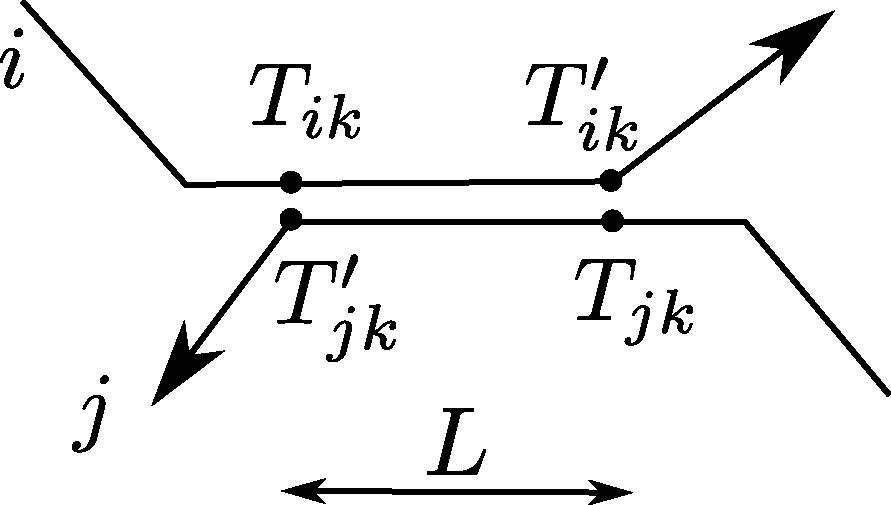
\includegraphics[width=0.3\linewidth]{pics/spatial_conflict_anti_parallel.pdf}
    \caption{Parallel and antiparallel spatial conflict}
    \label{fig:spatial_conflicts}
\end{figure}

\begin{itemize}
    \item {\bf Parallel conflict:}
        A real conflict exists if the difference between the arrival times is smaller than threshold $\Delta_p$ which depends on the trajectories, in particular the speed and position of both flights.
        \begin{equation*}
            \bigl| \underbrace{T_{jk} - T_{ik}}_{\Delta_k} \bigr| < \Delta_p
        \end{equation*}
        with
        \begin{equation*}
            \Delta_p = \Delta_p(v_i, v_j, r_i, r_j)
        \end{equation*}
        This can also be written as
        \begin{equation}  \label{eqn:spatial_conflict_parallel}
            \Delta_p > \Delta_k > -\Delta_p 
        \end{equation}
        
    \item {\bf Antiparallel conflict:}
        A real conflict exists if 
        \begin{equation*}
            T'_{ik} - T_{jk} > \Delta^1_{ap}(v_i, v_j, r_i, r_j)
        \end{equation*}
        and
        \begin{equation*}
            T'_{jk} - T_{ik} > \Delta^2_{ap}(v_i, v_j, r_i, r_j)
        \end{equation*}
        Hence
        \begin{eqnarray*}
            \frac{L_k}{v_i} + \underbrace{T_{ik} - T_{jk}}_{-\Delta_k} > \Delta^1_{ap} \\
            \frac{L_k}{v_j} + \underbrace{T_{jk} - T_{ik}}_{\Delta_k} > \Delta^1_{ap} 
        \end{eqnarray*}
        This yields
        \begin{equation} \label{eqn:spatial_conflict_antiparallel}
            \frac{L_k}{v_i} - \Delta^1_{ap} > \Delta_k > \Delta^2_{ap} - \frac{L_k}{v_j}
        \end{equation}
\end{itemize}

\subsection{Calculation of the conflict arrival times}
A classical precalculation gives us all spatial conflicts $k$, and therefore a mapping
\begin{equation*}
    k \mapsto \{i, j\} = I_k
\end{equation*}
We can get the spatial conflicts in which the flight $i$ is involved, ordered by their temporal appearance:
\begin{equation*}
    i \mapsto (k^i_1, \dots, k^i_{N_i})
\end{equation*}
We conflict avoiding maneuver delays the flight by a certain amount of time
\begin{equation*}
    d_{ik} \quad, \quad  k\in\{k^i_1, \dots, k^i_{N_i}\}
\end{equation*}
The arrival time of flight $i$ at conflict $k$ then reads
\begin{equation*}
    T_{ik} = t_{ik} + \sum_{p \in K^<_{ik}} d_{ip}
\end{equation*}
where the set of conflicts the flight $i$ was involved in before $k$ is given by
\begin{equation*}
    K^<_{ik} = \{\tilde k : \tilde k \in\{k^i_1, \dots, k^i_{N_i}\}, \tilde k < k\}
\end{equation*}
and $t_{ik}$ denotes the arrival time of flight $i$ at conflict $k$ in the absence of any delays, i.e. in the wind-optimal case.

\section{Independent delay model}
We assume, that the delays $d_{ik}$ are independent of each other. 
This means at every conflict $k \in  \{k^i_1, \dots, k^i_{N_i}\}$ for a given flight $i$, we can introduce a delay $d_{ik}$ which is independent of the delays of the other flights $d_{jk}$ for $j\neq i$.
Our goal is then to write down a cost function penalizes the total delay as well as the appearance of real conflicts (depending on the arrival times).
The departure delays $d_i$ can be seen as the result of a conflict $k^i_0$ at departure which only involved the flight itself.
\begin{equation*}
    d_i \to d_{ik^i_0}
\end{equation*}

The variables we try to optimize are the delays $d_{ik}$.
We bound and discretize the values they can assume by introducing binary variables $d_{ik\beta}\in\{0, 1\}$ :
\begin{equation*}
    d_{ik} = \Delta_d \sum_\beta \beta d_{ik\beta}
\end{equation*}
The total delay is given by
\begin{equation}
    D(\{d_{ik}\}) = \Delta_d \sum_k \sum_{i \in I_k} \sum_\beta \beta d_{ik\beta}
\end{equation}
The term which ensures the uniqueness of the variables $d_{ik}$ reads
\begin{equation}
    D^\text{one}(\{d_{ik}\})  =  \sum_k \sum_{i \in I_k} \left( \sum_\beta d_{ik\beta} - 1\right)^2
\end{equation}
In order to penalize the a real conflict, we need to write down the difference in the conflict arrival times in terms of the binary variables.
\begin{eqnarray*}
    \Delta_k &=& T_{ik} - T_{jk} \\
             &=& t_{ik} - t_{jk} + \Delta_d \left( \sum_\beta \sum_{p\in K^<_{ik}} \beta d_{ip\beta}  - \sum_\gamma \sum_{q\in K^<_{ik}} \gamma d_{iq\beta} \right)
\end{eqnarray*}
With \eqref{eqn:spatial_conflict_parallel} we have a real conflict in the parallel case if
\begin{equation*}
    \Delta_k \in [-\Delta_p, \Delta_p]
\end{equation*}
and in the antiparallel case \eqref{eqn:spatial_conflict_antiparallel} if
\begin{equation*}
    \Delta_k \in \left[\frac{L_k}{v_i} - \Delta^1_{ap}, \Delta^2_{ap} - \frac{L_k}{v_j}\right]
\end{equation*}

In order to penalize real conflicts, we could introduce $\Delta_k$ as a slack variable.
However, due to the unbounded region this variable assumes to avoid a conflict, the number of qubits would be very large.

\end{document}
